\documentclass[10pt]{article}

\usepackage[a4paper,margin=1in]{geometry}
\usepackage{times}
\usepackage{microtype}
\usepackage{graphicx}
\usepackage{booktabs}
\usepackage{array}
\usepackage{multirow}
\usepackage{tabularx}
\usepackage{enumitem}
\usepackage{xcolor}
\usepackage{tikz}
\usepackage{caption}
\usepackage{subcaption}
\usepackage[numbers,sort&compress]{natbib}
\usepackage[hidelinks]{hyperref}

\usetikzlibrary{arrows.meta,positioning,fit,calc}

\definecolor{agentblue}{HTML}{DBEAFE}
\definecolor{toolgreen}{HTML}{CCFBF1}
\definecolor{repairamber}{HTML}{FEF3C7}
\definecolor{textdark}{HTML}{111827}
\definecolor{bordergray}{HTML}{94A3B8}

\newcommand{\tool}[1]{\textsc{#1}}
\newcommand{\agent}[1]{\textsc{#1}}
\newcommand{\project}{SVG Icon Agent}

\title{\vspace{-1.8em}\textbf{\project: A Collaborative LLM-Agent Pipeline for Editable SVG Icon Generation}}
\author{
  Guanjie Zhao\\
  Student ID: 23307130127\\
  Fudan University\\
  \texttt{https://github.com/fwar1nben/CG\_PJ}
}
\date{}

\begin{document}
\maketitle

\begin{abstract}
This report presents \project, a course project for generative AI practice in computer graphics.
The system converts short English icon prompts into editable SVG assets through a collaborative LLM-agent pipeline rather than a raster text-to-image model.
It decomposes icon creation into goal management, local memory retrieval, prompt rewriting, structured planning, multi-candidate SVG drafting, semantic and SVG-quality critique, consensus selection, optimization, validation, failure taxonomy, repair routing, refinement, memory curation, and gallery export.
The graphics output remains inspectable as SVG source code, while deterministic local tools check parseability, safety, canvas constraints, primitive usage, rendering risk, and export artifacts.
In the current Web UI experiment snapshot, 15 single-prompt runs generated 45 candidate SVGs and 15 selected winners.
The optimized baseline icons were valid in 13/15 cases, while the final refined icons were valid in 15/15 cases; the average validation score improved from 89.33 to 93.20.
Code is available at \url{https://github.com/fwar1nben/CG_PJ}.
\end{abstract}

\section{Introduction}

Generative AI systems in graphics are often demonstrated through impressive raster images, 3D scenes, or videos.
However, many daily graphics tasks are smaller and more structural: a user may need a clean toolbar icon, a notification badge, a security symbol, or a simple object pictogram that can be edited after generation.
For these cases, the output format matters.
A PNG image can look attractive, but it is difficult to inspect, repair, recolor, or integrate into a design system.
An SVG icon, in contrast, exposes its geometry, colors, accessibility metadata, and canvas constraints directly as editable vector code \citep{svg11}.

\project{} explores this narrower but practical setting.
The project asks whether a language-model-driven agent workflow can generate usable editable SVG icons by decomposing the task into explicit subproblems.
Instead of asking one model call to ``draw an icon'', the system separates goal formation, prompt improvement, planning, candidate generation, independent critique, consensus selection, validation, and targeted repair.
This design follows a central observation from recent graphics agents: generation quality improves when high-level intent, intermediate structure, visual criticism, and repair strategy are represented explicitly \citep{genpilot2025,paper2poster2025,posterforest2025}.

The main contributions of this project are:
\begin{itemize}[leftmargin=1.5em,itemsep=0.2em]
  \item an end-to-end multi-agent workflow for editable text-to-SVG icon generation;
  \item a retrieval-augmented goal-conditioning step that reuses local historical run memories;
  \item a candidate--critic--selector stage that makes selection inspectable instead of relying on a single sample;
  \item a validation and repair loop with failure taxonomy and route selection before refinement;
  \item a Web UI that exposes agent progress, generated artifacts, raw traces, post-run optimizer feedback, and an SVG source editor.
\end{itemize}

\section{Related Work}

\paragraph{Prompt optimization and 2D generation agents.}
GenPilot decomposes text-to-image prompt optimization into error detection, prompt improvement, multi-candidate generation, scoring, and memory \citep{genpilot2025}.
PromptSculptor similarly studies multi-agent prompt optimization for image generation \citep{promptsculptor2025}.
These systems motivated the idea that visual generation should not be treated as a single opaque prompt-to-output call.
\project{} adapts this philosophy to SVG icon generation, where the output can be checked as source code and repaired structurally.

\paragraph{Layout and poster agents.}
Paper2Poster turns long scientific papers into posters through parsing, planning, layout, and visual feedback \citep{paper2poster2025}.
PosterForest further emphasizes hierarchical multi-agent collaboration for poster generation \citep{posterforest2025}.
Although this project targets icon-sized graphics rather than large posters, it shares the same principle: split graphics generation into content understanding, structured planning, rendering, critique, and revision.

\paragraph{Tool-augmented graphics agents.}
Agentic 3D and CAD systems such as CAD-Assistant show that language models become more useful for graphics tasks when they can interact with domain-specific tools and constraints \citep{cadassistant2025}.
\project{} follows this tool-augmented pattern in a lightweight 2D vector domain.
The LLM agents make semantic and design decisions, while local tools perform deterministic SVG checks, render previews, and export reports.

\section{Method}

\subsection{Task Definition}

The input is a short English prompt describing an icon, such as a rocket launch icon, a steaming coffee cup, or a security shield.
The desired output is a complete SVG file that is:
\begin{itemize}[leftmargin=1.5em,itemsep=0.2em]
  \item valid XML/SVG with a square canvas and explicit \texttt{viewBox};
  \item editable through standard SVG primitives and paths;
  \item safe, with no scripts, external references, iframes, animation tags, or foreign objects;
  \item visually recognizable at small icon sizes;
  \item exported with PNG previews, validation reports, traces, and gallery pages.
\end{itemize}

\subsection{Agent Pipeline}

Figure~\ref{fig:pipeline} shows the core workflow.
Named agents call the configured LLM backend through OpenRouter \citep{openrouter}; deterministic local modules are treated as tools rather than agents.
The default model configured in the project is \texttt{openai/gpt-oss-120b:free}.

\begin{figure}[t]
\centering
\resizebox{\linewidth}{!}{
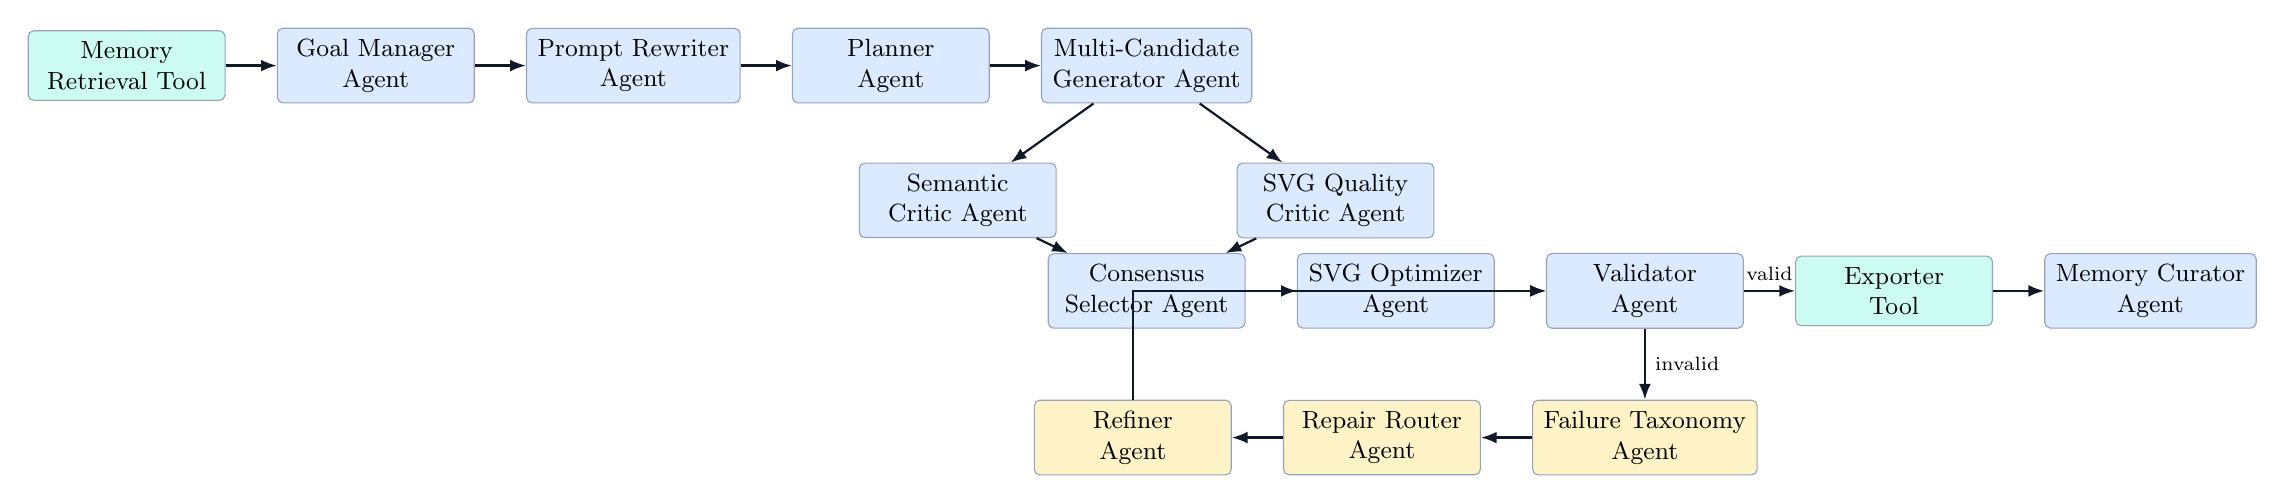
\begin{tikzpicture}[
  node distance=0.55cm and 0.65cm,
  every node/.style={font=\small,align=center},
  agentnode/.style={draw=bordergray,rounded corners=2pt,fill=agentblue,inner sep=4pt,minimum width=2.5cm,minimum height=0.75cm},
  toolnode/.style={draw=bordergray,rounded corners=2pt,fill=toolgreen,inner sep=4pt,minimum width=2.5cm,minimum height=0.75cm},
  repairnode/.style={draw=bordergray,rounded corners=2pt,fill=repairamber,inner sep=4pt,minimum width=2.5cm,minimum height=0.75cm},
  arrow/.style={-{Latex[length=2mm]},thick,draw=textdark}
]
\node[toolnode] (memory) {Memory\\Retrieval Tool};
\node[agentnode,right=of memory] (goal) {Goal Manager\\Agent};
\node[agentnode,right=of goal] (rewrite) {Prompt Rewriter\\Agent};
\node[agentnode,right=of rewrite] (planner) {Planner\\Agent};
\node[agentnode,right=of planner] (generator) {Multi-Candidate\\Generator Agent};

\node[agentnode,below left=0.75cm and -0.2cm of generator] (semantic) {Semantic\\Critic Agent};
\node[agentnode,below right=0.75cm and -0.2cm of generator] (quality) {SVG Quality\\Critic Agent};
\node[agentnode,below=1.9cm of generator] (selector) {Consensus\\Selector Agent};
\node[agentnode,right=of selector] (optimizer) {SVG Optimizer\\Agent};
\node[agentnode,right=of optimizer] (validator) {Validator\\Agent};

\node[repairnode,below=0.9cm of validator] (taxonomy) {Failure Taxonomy\\Agent};
\node[repairnode,left=of taxonomy] (router) {Repair Router\\Agent};
\node[repairnode,left=of router] (refiner) {Refiner\\Agent};
\node[toolnode,right=of validator] (exporter) {Exporter\\Tool};
\node[agentnode,right=of exporter] (curator) {Memory Curator\\Agent};

\draw[arrow] (memory) -- (goal);
\draw[arrow] (goal) -- (rewrite);
\draw[arrow] (rewrite) -- (planner);
\draw[arrow] (planner) -- (generator);
\draw[arrow] (generator) -- (semantic);
\draw[arrow] (generator) -- (quality);
\draw[arrow] (semantic) -- (selector);
\draw[arrow] (quality) -- (selector);
\draw[arrow] (selector) -- (optimizer);
\draw[arrow] (optimizer) -- (validator);
\draw[arrow] (validator) -- node[right,font=\scriptsize]{invalid} (taxonomy);
\draw[arrow] (taxonomy) -- (router);
\draw[arrow] (router) -- (refiner);
\draw[arrow] (refiner) |- (validator);
\draw[arrow] (validator) -- node[above,font=\scriptsize]{valid} (exporter);
\draw[arrow] (exporter) -- (curator);
\end{tikzpicture}
}
\caption{The \project{} workflow. Blue nodes are LLM-backed agents, green nodes are deterministic tools, and yellow nodes form the conditional repair route.}
\label{fig:pipeline}
\end{figure}

\subsection{Retrieval and Goal Conditioning}

The \tool{Memory Retrieval Tool} searches local memory records from previous runs.
Each memory record contains a prompt summary, successful strategies, failure patterns, user feedback, tags, and scores.
The \agent{Goal Manager Agent} then converts the raw user prompt, optional user goal, and retrieved memory context into explicit objectives, visual requirements, constraints, acceptance criteria, preferences, and avoid patterns.
This step makes the generation target observable before any SVG is drafted.

\subsection{Planning, Candidate Generation, and Critique}

The \agent{Prompt Rewriter Agent} rewrites the user input into a concise SVG-icon prompt.
The \agent{Planner Agent} extracts an icon category, motifs, palette, layout, and constraints.
The \agent{Multi-Candidate Generator Agent} then produces three distinct SVG drafts for each prompt in collaborative mode.
Two independent critics evaluate the candidates:
\begin{itemize}[leftmargin=1.5em,itemsep=0.2em]
  \item the \agent{Semantic Critic Agent} scores prompt alignment, recognizability, and small-size readability;
  \item the \agent{SVG Quality Critic Agent} scores editability, safety, rendering risk, and deterministic SVG check issues.
\end{itemize}
The \agent{Consensus Selector Agent} selects the strongest draft and writes a repair brief for downstream optimization.

\subsection{Optimization, Validation, and Repair}

The selected SVG is not immediately accepted.
The \agent{SVG Optimizer Agent} rewrites it using critic reports, selector risks, deterministic tool findings, and optional human feedback.
The \agent{Validator Agent} then judges semantic alignment, visual quality, editability, and rule compliance.
If validation finds blocking issues, the pipeline invokes:
\begin{enumerate}[leftmargin=1.5em,itemsep=0.2em]
  \item the \agent{Failure Taxonomy Agent}, which classifies failure types and root causes;
  \item the \agent{Repair Router Agent}, which chooses an ordered repair strategy such as safety rebuild, semantic recomposition, simplification, layout rebalance, or minor patch;
  \item the \agent{Refiner Agent}, which returns a complete repaired SVG.
\end{enumerate}
The repaired SVG is sent back to validation until accepted or the configured repair-round limit is reached.

\section{Implementation}

The implementation is a Python project organized around the \texttt{svg\_icon\_agent} package.
The CLI entry point supports JSON prompt cases, selected cases, manual text prompts, and interactive prompts.
The Web UI writes timestamped runs under \texttt{outputs/web/}, exposes live agent states, displays candidate/selected/baseline/refined SVGs, and provides a source-level SVG editor that saves separate edited artifacts without overwriting generated outputs.

Local code intentionally does not synthesize fallback icons when a model call fails.
Instead, it records errors in trace files so that failures remain inspectable.
The deterministic toolchain performs prompt loading, memory retrieval, SVG safety and structure checks, PNG rendering, metric aggregation, HTML gallery export, and raw response logging.
Generated outputs include candidate SVGs, selected SVGs, optimized baselines, refined SVGs, PNG previews, validation JSON, failure taxonomies, repair routes, memory context, generation goals, LLM traces, and raw LLM response logs.

\section{Experiments and Results}

\subsection{Setup}

The current evaluation uses the completed Web UI runs under \texttt{outputs/web/}.
Each run is a single-prompt icon generation case using collaborative mode with three candidates.
The snapshot includes 15 runs, 45 candidate SVG drafts, and 15 selected winners.
This is a small project evaluation intended to verify the full workflow, not a large-scale benchmark.

The main metrics are baseline validity, final refined validity, validation score, score delta, and maximum repair rounds.
The baseline is the optimized SVG after candidate selection and optimizer feedback.
The refined result is the output after conditional validation and repair.

\begin{table}[t]
\centering
\caption{Current Web UI experiment snapshot.}
\label{tab:metrics}
\begin{tabular}{lr}
\toprule
Metric & Value \\
\midrule
Web UI single-prompt runs & 15 \\
Generated candidate SVGs & 45 \\
Selected winners & 15 \\
Valid optimized baselines & 13/15 \\
Valid final refined icons & 15/15 \\
Baseline average validation score & 89.33 \\
Refined average validation score & 93.20 \\
Average score delta & +3.87 \\
Maximum repair rounds used & 3 \\
\bottomrule
\end{tabular}
\end{table}

\subsection{Repair Examples}

Table~\ref{tab:cases} lists representative repair cases from the run logs.
The coffee and dog cases show the clearest effect of the validation--taxonomy--routing--refinement loop.
The apple case is included as an honest caveat: a refined result can be accepted while receiving a lower validation score, which suggests that future work should combine automatic validation with human preference evaluation.

\begin{table}[t]
\centering
\caption{Representative validation-score changes after repair.}
\label{tab:cases}
\begin{tabularx}{\linewidth}{lrrrl}
\toprule
Case & Baseline & Refined & Rounds & Observation \\
\midrule
Steaming coffee cup & 70 & 95 & 1 & Large semantic and visual repair gain \\
Cute yellow dog & 65 & 100 & 1 & Strong improvement after targeted refinement \\
Clean line icon & 88 & 95 & 3 & Multi-round repair improves structure \\
Apple icon & 85 & 70 & 1 & Accepted but lower score; metric caveat \\
\bottomrule
\end{tabularx}
\end{table}

\subsection{Generated Examples}

Figure~\ref{fig:examples} shows generated refined icons selected from the project outputs.
The examples cover object icons, UI symbols, education/productivity symbols, and simple scene-like icons.
They demonstrate that the system can create compact vector assets with clean silhouettes and small-size readability.

\begin{figure}[t]
\centering
\begin{subfigure}{0.115\linewidth}
\centering

\includegraphics[width=\linewidth]{figures/gen_rocket.png}
\caption*{\scriptsize Rocket}
\end{subfigure}
\begin{subfigure}{0.115\linewidth}
\centering

\includegraphics[width=\linewidth]{figures/gen_coffee.png}
\caption*{\scriptsize Coffee}
\end{subfigure}
\begin{subfigure}{0.115\linewidth}
\centering

\includegraphics[width=\linewidth]{figures/gen_dog.png}
\caption*{\scriptsize Dog}
\end{subfigure}
\begin{subfigure}{0.115\linewidth}
\centering

\includegraphics[width=\linewidth]{figures/gen_book.png}
\caption*{\scriptsize Book}
\end{subfigure}
\begin{subfigure}{0.115\linewidth}
\centering

\includegraphics[width=\linewidth]{figures/gen_landscape.png}
\caption*{\scriptsize Scene}
\end{subfigure}
\begin{subfigure}{0.115\linewidth}
\centering

\includegraphics[width=\linewidth]{figures/gen_cloud.png}
\caption*{\scriptsize Cloud}
\end{subfigure}
\begin{subfigure}{0.115\linewidth}
\centering

\includegraphics[width=\linewidth]{figures/gen_shield.png}
\caption*{\scriptsize Shield}
\end{subfigure}
\begin{subfigure}{0.115\linewidth}
\centering

\includegraphics[width=\linewidth]{figures/gen_calendar.png}
\caption*{\scriptsize Calendar}
\end{subfigure}
\caption{Example refined icon outputs used for visual inspection in the project report and presentation materials.}
\label{fig:examples}
\end{figure}

\section{Discussion and Limitations}

The experiment suggests that an agentic SVG workflow can improve validity and inspectability compared with accepting the first generated draft.
The explicit repair loop is especially useful when the baseline icon is semantically close but structurally flawed, visually cluttered, or unsafe.
The Web UI also makes the system easier to demonstrate because users can inspect rewritten prompts, retrieved memory, candidates, selected winners, validation issues, repair routes, raw responses, and final SVG source.

Several limitations remain.
First, the current evaluation is small: 15 single-prompt Web runs are enough to validate the workflow but not enough for a robust benchmark.
Second, the validation score is LLM-assisted and should be complemented by human preference studies.
Third, the local \tool{SvgCheckTool} covers a practical safe subset of SVG rather than the entire SVG standard.
Fourth, the system depends on the availability and quality of the configured LLM service; free API models can be slow, rate-limited, or inconsistent.
Finally, the current generator focuses on simple icon graphics rather than complex illustration, typography, or full layout design.

\section{Conclusion}

\project{} demonstrates a practical agent-based approach to editable vector graphics generation.
By decomposing text-to-SVG icon creation into goal conditioning, prompt rewriting, planning, candidate generation, critique, selection, optimization, validation, taxonomy, routing, and refinement, the system makes generation more inspectable and repairable.
The current project snapshot improves valid icons from 13/15 optimized baselines to 15/15 final refined results, with an average validation-score increase from 89.33 to 93.20.
Future work should expand the prompt set, add human preference evaluation, compare more ablation settings such as single-shot generation and no-memory generation, and broaden the SVG grammar while preserving safety and editability.

\section*{Member Contributions}

\textbf{Guanjie Zhao} (Student ID: \textbf{23307130127}) completed this as a solo project.
The work included topic selection, system design, implementation of the multi-agent SVG pipeline, Web UI development, SVG editor integration, experiment execution, evaluation, artifact organization, report writing, and presentation preparation.

\bibliographystyle{plainnat}
\bibliography{references}

\end{document}
